% !TEX root = main.tex

\documentclass{beamer}
\usepackage{listings}
\usepackage{booktabs}
\usepackage{bookmark}
\usepackage[spanish]{babel}
\usepackage{makecell}
\usepackage{url}
\usepackage{multirow}
\usepackage{graphicx}
\usepackage{amsmath, amsthm, amssymb}

\usepackage{beamerthemesplit}
\usetheme{Marburg}
\usecolortheme{dolphin}

\lstdefinestyle{latexStyle}{
    language=[LaTeX]{TeX},
    belowcaptionskip=1\baselineskip,
    breaklines=true,
    frame=none,
    numbers=none, 
    basicstyle=\footnotesize\ttfamily,
    keywordstyle=\bfseries\color{green!40!black},
    commentstyle=\itshape\color{purple!40!black},
    identifierstyle=\color{blue},
    backgroundcolor=\color{gray!10!white},
}
\lstset{style=latexStyle}

\title{Moogle!}

\institute{MATCOM}
\author{Jossué Arteche Muñoz, C111}
\date{Julio, 2023}

\begin{document}
\maketitle

\section{Introducción}\label{intro}

\begin{frame}
    \begin{columns}[t]
        \begin{column}{.5\textwidth}
          \tableofcontents[sections={1-2},currentsection]
        \end{column}
        \begin{column}{.5\textwidth}
          \tableofcontents[sections={3-4},currentsection]
        \end{column}
    \end{columns}
\end{frame}

\subsection{¿Qué es Moogle!?}
\begin{frame}{¿Qué es Moogle!?}
\begin{center}
El proyecto “Moogle!” es una aplicación cuyo propósito es buscar inteligentemente un texto en un conjunto de documentos. 

\begin{figure}[h]
    \center
    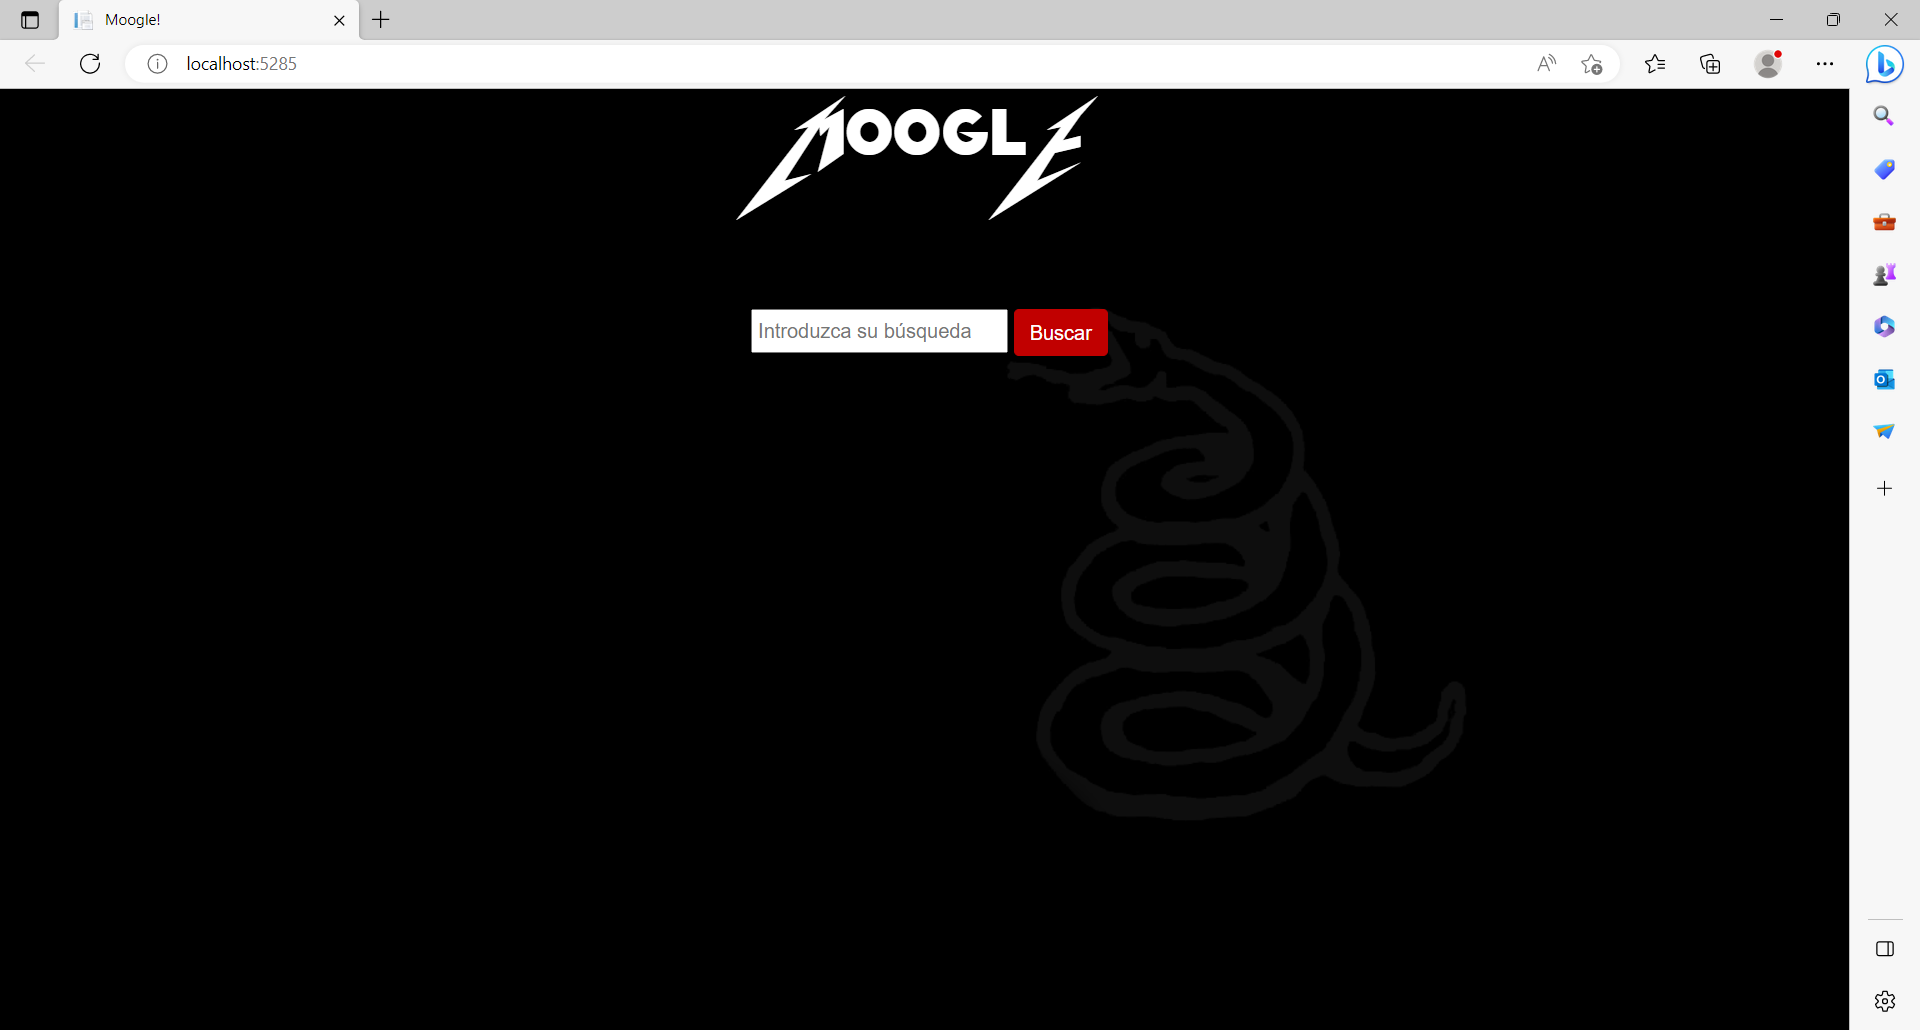
\includegraphics[width=5cm]{interfaz.png}
    \caption{Interfaz de Moogle!}
\end{figure}

\end{center}

\end{frame}


\subsection{Características}
\begin{frame}{Características}

Características:
\begin{itemize}
  \item Realiza búsquedas en un conjunto de documentos
  \item Devuelve resultados organizados por relevancia y de manera rápida
  \item Admite operadores de búsqueda básicos
  \item Muestra un snippet y realiza sugerencias
\end{itemize}

\end{frame}




\section{Funcionamiento general}

\begin{frame}
    \begin{columns}[t]
        \begin{column}{.5\textwidth}
          \tableofcontents[sections={1-2},currentsection]
        \end{column}
        \begin{column}{.5\textwidth}
          \tableofcontents[sections={3-4},currentsection]
        \end{column}
    \end{columns}
\end{frame}

\subsection{Bases del funcionamiento}
\begin{frame}[fragile]{}

Moogle! se basa principalmente en:
\begin{itemize}
\item Modelo Vectorial
\item Tf-Idf
\item Similitud Coseno

\end{itemize}

\pause
\vspace{5mm}
¿Pero, en qué consiste cada uno?

\end{frame}

\subsection{Modelo Vectorial}
\begin{frame}[fragile]{Modelo Vectorial}

El modelo vectorial se basa expresar cada
documento como vectores de la misma dimension usando la relevancia de cada palabra
\pause

\begin{figure}[h]
    \center
    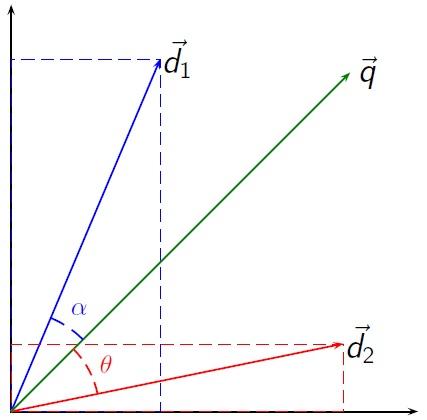
\includegraphics[width=4cm]{Vectormodel.jpg}
    \caption{Modelo Vectorial}
\end{figure}

\end{frame}

\subsection{Tf-Idf}
\begin{frame}[fragile]{Tf-Idf}

Term frecuency – Inverse term frecuency, es un valor que se utiliza para calcular la relevancia de cada palabra.


\pause
$ tf(t,d) $: cantidad de veces que aparece el término $t$ en el documento $d$ del conjunto de documentos $D$ 
%aqui va la formulita
\begin{equation}
    idf(t,D) = \log{\frac{|D|}{|\{d\in{D}:t\in{d}\}|}}
\end{equation}
\begin{equation}
    tfidf(t,d,D) = tf(t,d)*idf(t,D)
\end{equation}


\end{frame}

\subsection{Similitud Coseno}
\begin{frame}{Similitud Coseno}

La similitud consiste en calcular la relevancia entre dos de los vectores (documentos) a partir del valor del coseno del ángulo comprendido
\pause

\begin{figure}[h]
    \center
    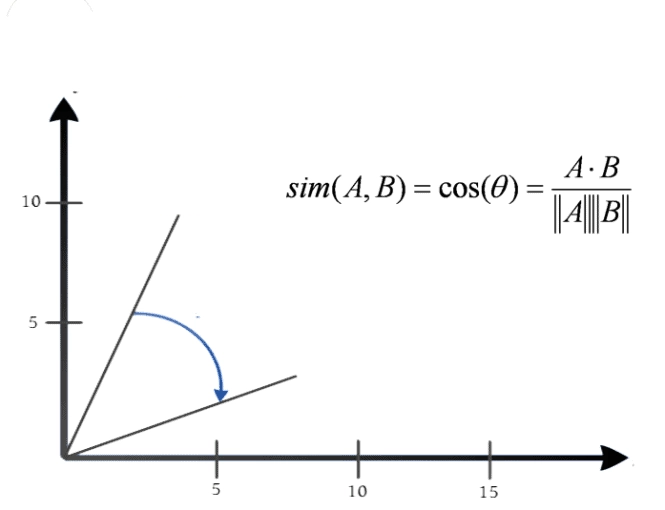
\includegraphics[width=6cm]{cosinesimilarity.png}
    \caption{Similitud Coseno}
\end{figure}

\end{frame}



\section{Estructura del Funcionamiento}
\begin{frame}
    \begin{columns}[t]
        \begin{column}{.5\textwidth}
          \tableofcontents[sections={1-2},currentsection]
        \end{column}
        \begin{column}{.5\textwidth}
          \tableofcontents[sections={3-4},currentsection]
        \end{column}
    \end{columns}
\end{frame}

\subsection{Cálculos previos}
\begin{frame}[fragile]{Cálculos previos}
  Antes de realizar las primeras búsquedas se construye un objeto asociado a nuestra base de documentos

\end{frame}
\begin{frame}[fragile]{Almacenando Datos}
Se crea una estructura que relaciona cada palabra y los documentos
en los que aparece, y a su vez relaciona estos con las posiciones en
las que aparece cada palabra en dicho documento.

\pause

Para esto se usa un diccionario de diccionarios.
\end{frame}

\begin{frame}[fragile]{Alamcenando Datos}
Se crea cada vector documento, calculando el
tf-idf de cada palabra con funciones que estan implementadas dentro de una
clase TfIdfDirectory, de forma muy sencilla.
\pause

\begin{figure}[h]
    \center
    \includegraphics[width=10cm]{RepresentacionDelPreCalculo.png}
    \caption{Precálculo}
\end{figure}

\end{frame}

\subsection{Búsquedas}
\begin{frame}{Haciendo Búsquedas}

Cuando se introduce una búsqueda, esta se convierte en un vector ndimensional,
y se calcula su similitud coseno con todos los vectores documento.
Luego se seleccionan los 5 documentos de mayor similitud y se devuelven
como resultado.
\pause

\begin{figure}[h]
    \center
    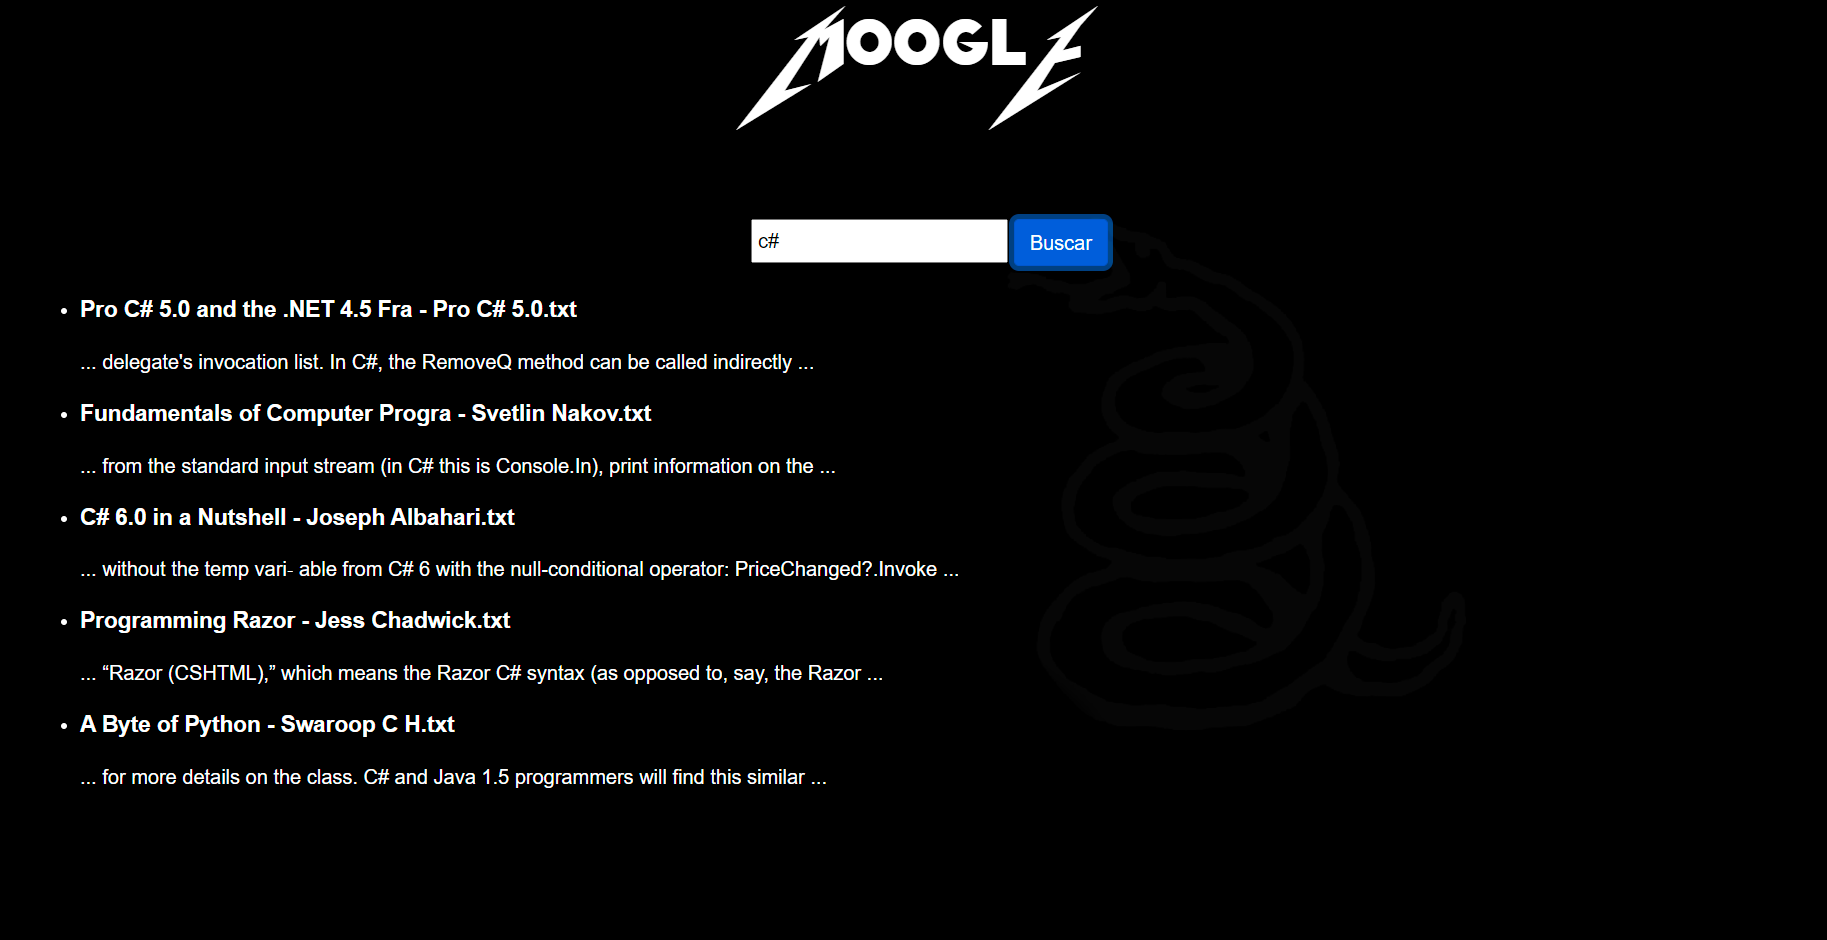
\includegraphics[width=6cm]{busqueda.png}
    \caption{Ejemplo de una búsqueda}
\end{figure}

\end{frame}

\begin{frame}[fragile]{Haciendo Búsquedas}

\begin{figure}[h]
    \center
    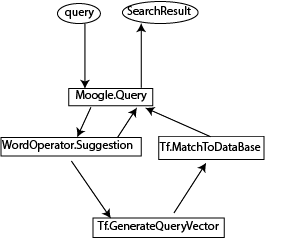
\includegraphics[width=7cm]{DiagramaDeClases.png}
    \caption{Proceso de respuesta}
\end{figure}

\end{frame}

\section{Otras Funcionalidades}

\begin{frame}
    \begin{columns}[t]
        \begin{column}{.5\textwidth}
          \tableofcontents[sections={1-2},currentsection]
        \end{column}
        \begin{column}{.5\textwidth}
          \tableofcontents[sections={3-4},currentsection]
        \end{column}
    \end{columns}
\end{frame}

\subsection{Operadores de Búsqueda}
\begin{frame}[fragile]{Operadores de Búsqueda}
Al realizar búsquedas con Moogle! se pueden usar operadores

\begin{itemize}
\item El caracter ```!'' excluye palabras de los resultados
\item Escribir ``\^{}'' antes de una palabra hará que los resultados la contengan
\item ``*'' antes de palabra, una o varias veces, aumenta la relevancia de esa palabra
\item Usar ``\~{}'' entre dos palabras devolvera los documentos en los que estas aparezcan cerca
\end{itemize}
\pause

En dependencia de la operación de cada palabra se juega con la similitud coseno para obtener los resultados esperados 

\end{frame}

\subsection{Snippet}
\begin{frame}[fragile]{Snippet}
Se toma la palabra mas relevante de la query y se busca la mediana de las posiciones en
las que se eencuentra de aparecer en el documento y se toma un fragmento
que tiene a dicha palabra en el centro.

\begin{figure}[h]
    \center
    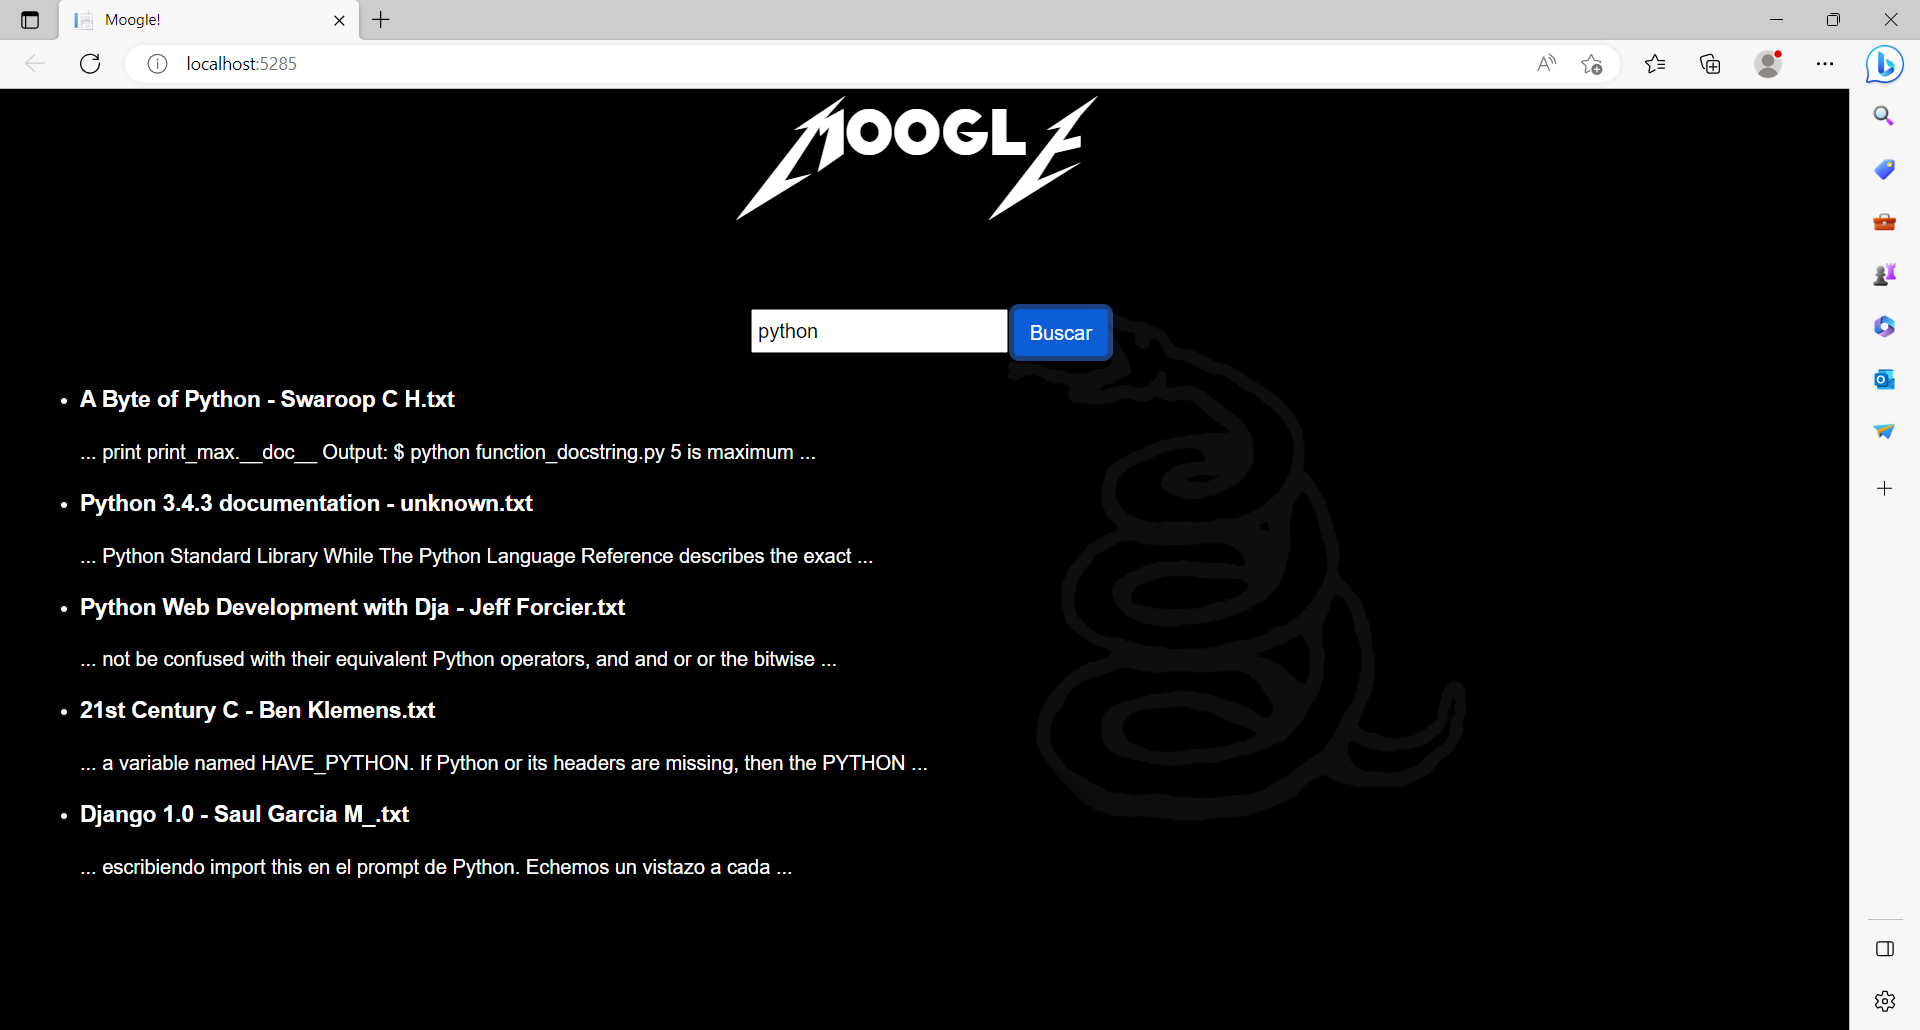
\includegraphics[width=6cm]{busqueda2.png}
    \caption{Debajo de cada resultado aparece el snippet}
\end{figure}

\end{frame}

\subsection{Sugerencias}
\begin{frame}[fragile]{Sugerencias}
En caso de que se una palabra que no se encuentre en el directorio entonces se busca
la palabra que contenga mas similar (usando distancia de levenshtein), luego se sustituye esa
posible palabra en la query y se vuelve a realizar la busqueda, obteniendo los
resultados sugeridos.

\begin{figure}[h]
    \center
    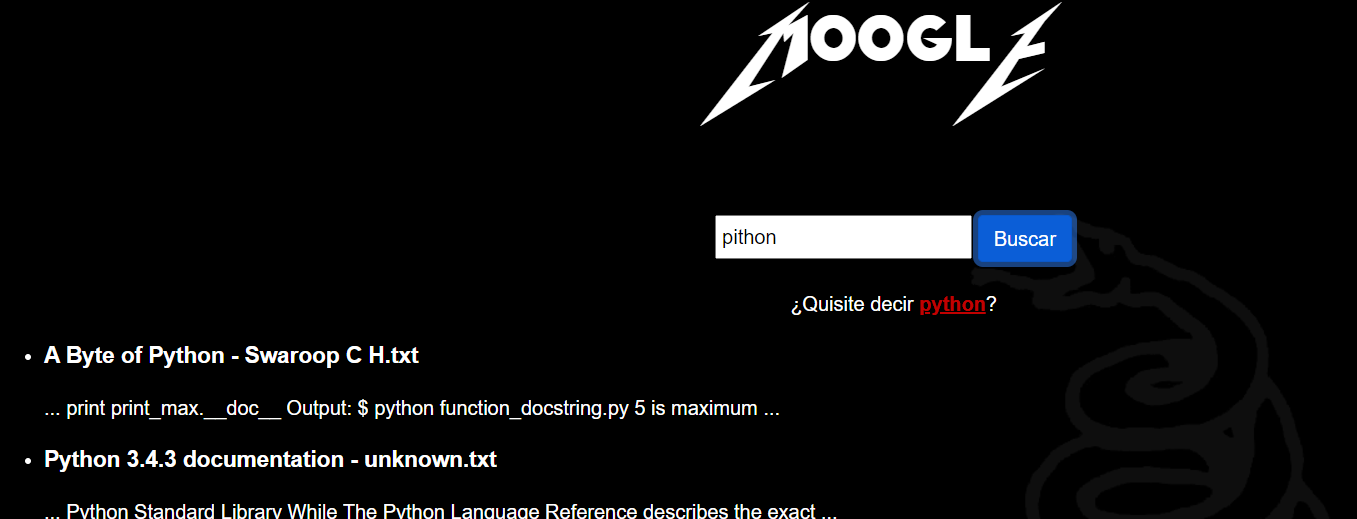
\includegraphics[width=8cm]{sugerencia.png}
    \caption{Ejemplo de Sugerencia}
\end{figure}

\end{frame}

\section{Clases Implementadas}

\begin{frame}
    \begin{columns}[t]
        \begin{column}{.5\textwidth}
          \tableofcontents[sections={1-2},currentsection]
        \end{column}
        \begin{column}{.5\textwidth}
          \tableofcontents[sections={3-4},currentsection]
        \end{column}
    \end{columns}
\end{frame}

\subsection{Clases Implementadas}
\begin{frame}[fragile]{Clases Implementadas}

\begin{itemize}
	\item Moogle
	\item WordsIndexer
	\item WordOperator
	\item TfIdfDirectory
	\item QueryDimension
	\item SimilarityResult
	\item WordOperation
\end{itemize}
\end{frame}


\maketitle
\end{document}
